\documentclass[a4paper,14pt]{extarticle}
\usepackage[russian]{babel}
\usepackage[colorlinks=False]{hyperref}
\usepackage[utf8]{inputenc}
\usepackage[margin=1.5cm,left=2cm,right=1cm]{geometry} % сделать по ГОСТУ
\usepackage{indentfirst}
\usepackage{graphicx}
\usepackage{amsmath}
\usepackage{multirow}
\usepackage{pgfplots}
\usepgfplotslibrary{fillbetween}

\usepackage{tikz}
\usetikzlibrary{circuits.ee.IEC}

\usepackage{circuitikz}
\ctikzset{bipoles/length=.8cm}

\tikzset{component/.style={draw,thick,circle,fill=white,minimum size =0.8cm,inner sep=0pt}}

\renewcommand{\small}{\fontsize{12pt}{14.4pt}\selectfont}
\usepackage{caption}
\DeclareCaptionLabelFormat{figure}{Рисунок #2}
\DeclareCaptionLabelFormat{table}{Таблица #2}
\DeclareCaptionLabelSeparator{sep}{~---~}
\captionsetup{labelsep=sep,justification=centering,font=small}
\captionsetup[figure]{labelformat=figure}
\captionsetup[table]{labelformat=table}

\usepackage{titlesec}
\titleformat{\section}
    {\centering\normalsize}
    {\thesection}
    {1em}{}
\titleformat{\subsection}
    {\centering\normalsize}
    {\thesubsection}
    {1em}{}
\titleformat{\subsubsection}
    {\centering\normalsize}
    {\thesubsubsection}
    {1em}{}

\titlespacing*{\section}{\parindent}{*4}{*1}
\titlespacing*{\subsection}{\parindent}{*4}{*1}
\titlespacing*{\subsubsection}{\parindent}{*4}{*1}

\renewcommand{\tan}{\mathrm{tg\,}}
\renewcommand{\baselinestretch}{1.5}

\parindent=1.25cm
\usepackage{enumitem}
\makeatletter
\AddEnumerateCounter{\asbuk}{\@asbuk}{м)}
\makeatother
\setlist{nosep,wide}

\tolerance=10000

\begin{document}
	\begin{titlepage}
        \begin{center}
          Министерство образования и науки Российской Федерации \\
          Федеральное государственное бюджетное образовательное \\
          учреждение высшего образования \\
          <<Волгоградский государственный технический университет>> \\
          Факультет электроники и вычислительной техники\\
          Кафедра <<Физика>>
        \end{center}
        \vspace{9em}
        \begin{center}
          \large
            Методические указания к лабораторной работе\\
            <<Исследование характеристик отражательного клистрона>>
        \end{center}
        \vspace{5em}
        \begin{flushright}
          \begin{minipage}{.40\textwidth}
            Выполнили:\\
            студенты группы Ф-2н\\
            Абдрахманов В. Л.\\
            Аликов С. А.\\
            \vspace{1em}\\
            Проверил:\\
            д.ф.-м.н., профессор\\
            Шеин А. Г.
          \end{minipage}
        \end{flushright}
        \vspace{\fill}
        \begin{center}
          Волгоград, \the\year
        \end{center}
    \end{titlepage}
    \setcounter{page}{2}

	\section*{Введение}
	В данной работе определяются <<горячие>> характеристики отражательного клистрона: его рабочая частота и добротность резонатора.
	
	\section{Теоретическая часть}
	\subsection{Устройство отражательного клистрона и принцип его работы}
	Отражательный клистрон представляет собой резонансный генератор колебаний СВЧ малой мощности.
	Работа отражательного клистрона основана на кратковременном взаимодействии электрического поля резонатора с электронным потоком. 
	Электроны,  эмитируемые  катодом,  ускоряются  в  пространстве  между катодом и резонатором, к которому приложено ускоряющее напряжение $U_0$.
	
	Возникающее между сетками резонатора CBЧ-напряжение $U(t)=U_m \sin \omega t$ производит модуляцию скорости электронов. В кинетической
	теории клистрона доказывается следующее приближённое выражение для скорости на выходе из модулирующего промежутка:
	\begin{equation}
	v = v_0 \left(1 + \frac{U_m}{2U_0} \beta \sin \left(\omega t_0 + \frac{\Phi}{2}\right) \right) = v_0 \left(1 + X \sin \left(\omega t_0 + \frac{\Phi}{2}\right) \right) ,
	\end{equation}
	где $v_0$, $t_0$~-- скорость электронов на влёте в резонатор и время влёта в резонатор соответственно, скорость определяется положительным потенциалом $U_0$ на резонаторе:
	\[
	\frac{mv_0^2}{2} = e U_0,
	\]
	$m$ и $e$ соответственно масса и абсолютное значение заряда электрона, $\beta$~-- параметр эффективной модуляции:
	\[
	\beta = \frac{\sin \cfrac{\Phi}{2}}{\cfrac{\Phi}{2}},
	\]
	$\Phi = d\omega/v_0$ угол пролёта электрона через высокочастотный зазор, $d$~-- расстояние между сетками резонатора.
	После вылета из резонатора электроны, двигаясь равнозамедленно в тормозящем поле отражателя $(U_0 + |U_r|)/l$, где $U_r$~-- потенциал отражателя, $l$~-- расстояние от резонатора до отражателя, уменьшают свою скорость до нулевого значения, затем начинают обратное движение и возвращаются в резонатор. В процессе этого движения к отражателю и обратно из-за различия скоростей электронов происходит образование сгустков. Движение в тормозящем поле происходит по параболам. Обозначив время вылета из резонатора $t_1$, получим уравнения траекторий в виде:
	\begin{equation}
	z = v (t - t_1) - \frac{e(U_0 + |U_r|)}{2ml} (t - t_1)^2.
	\end{equation}
	Найдём время возвращения в резонатор. Очевидно, что оно равно:
	\begin{equation}
	t_2 = t_1 +  v \frac{2ml}{e(U_0 + |U_r|)}.
	\end{equation}
	
	Чтобы  образовавшиеся  электронные  сгустки  отдавали  энергию  СВЧ-полю и поддерживали колебания в резонаторе, они должны возвращаться в резонатор в тормозящий полупериод. Для этого необходимо, как это видно из пространственно-временной диаграммы (рисунок \ref{cond}),  чтобы  сгустки  электронов  возвращались  в  резонатор  через целое число периодов без одной четверти, т.е. 
	$$ \omega (t_2 - t_1) = 2\pi \left(n + \frac{3}{4}\right)$$
	где n = 0, 1, 2, 3, 4, ... 
	
	\begin{figure}[h]
		\center
		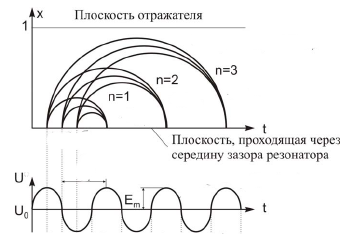
\includegraphics[width = 0.6\textwidth]{images/12.png}
		\caption{Условие генерации}
		\label{cond}
	\end{figure}
	
	Отсюда следует формула для расчёта зон генерации:
	\begin{equation}
	n \approx \frac{\omega mlv_0}{\pi e(U_0 + |U_r|)} - \frac{3}{4} \approx \sqrt{\frac{2m}{e}}\frac{\omega l\sqrt{U_0}}{\pi (U_0 + |U_r|)} - \frac{3}{4}.
    \label{eq:n}
	\end{equation}
	
	Воспользовавшись представлениями об эквивалентной схеме клистрона [1, 2, 3] или более точным методом, в котором решается уравнение возбуждения [2, 4], можно получить следующие соотношения для частоты генерируемого сигнала $f$ и его мощности $P$ (рисунок \ref{figz}):
	\begin{gather}
	f = f_0 \left(1 - \frac{1}{2Q} \tan \left( \frac{2\pi(n + 3/4)}{U_0 + |U_r|} \delta U_r \right)\right), \label{eq:Q}\\
	P = I_0 U_0 \frac{\cos (2\pi (n + 3/4)\delta U_r/(U_0 + |U_r|)}{\pi (n + 3/4)} X J_1(X),
	\end{gather}
	где $f_0 = \omega/2\pi$~-- частота соответствующая центру зоны генерации, $Q$~-- добротность резонатора, $\delta U_r$~-- перестройка напряжения от центра зоны генерации, $I_0$~-- ток резонатора, $J_1(X)$~-- функция Бесселя первого порядка, $X = U_m\beta/2U_0$~-- параметр модуляции. Отсюда следует, что для определения добротности резонатора необходимо определить перестройку частоты в малом диапазоне напряжений отражателя в окрестности центра зоны генерации.
	
	\begin{figure}[h]
		\center
		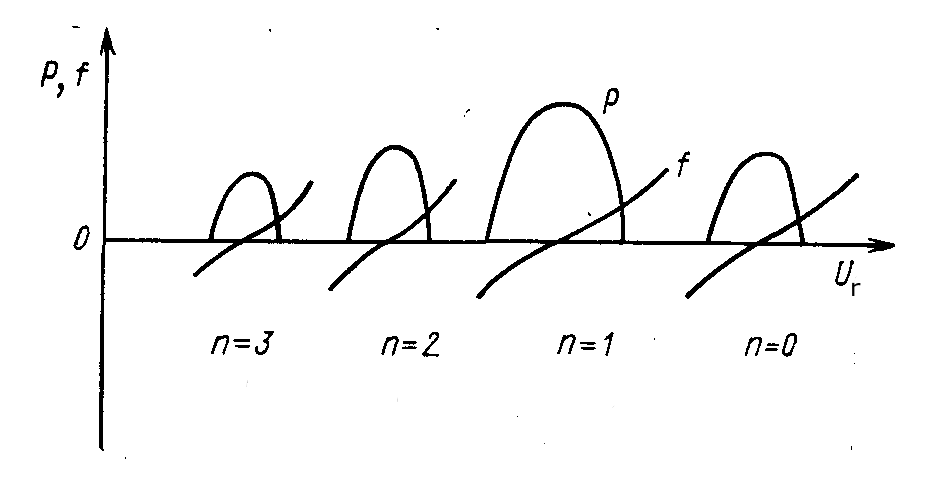
\includegraphics[width = 0.7\textwidth]{images/zones.png}
		\caption{Зоны генерации, мощность и перестройка частоты внутри зоны}
		\label{figz}
	\end{figure}

	\section{Методика проведения измерений}
	\subsection{Описание установки}
	В работе используются следующие приборы: клистрон, блок питания клистрона, анализатор спектра С4-27, генератор импульсов Г?-??, осциллограф С?-??, измерительная линия ??-??, усилитель пилообразного сигнала, а также соединительные элементы (коаксиальный кабель, 2 волноводно\-коаксиальных переходника, коаксиальные аттенюаторы (используются при необходимости)). Последовательно собираются две схемы измерений.
	
	Первая схема измерений предназначена для определения напряжений отражателя, соответствующих зонам генерации. Она представлена на рисунке (! перерисовать с усилителем пилы, импульсным генератором, линией и осциллографом) \ref{sch1}.
    \begin{figure}[h]
        \center
        \begin{tikzpicture}
            \begin{scope}
                % корпус
                \draw (-1, -1) -- (-1, 1);
                \draw (1, -1) -- (1, 1);
                \draw (1, 1) arc (0:180:1 and 0.7); 
                \draw (-1, -1) arc (180:360:1 and 0.7);
                % резонатор (выход)
                \draw (0.7, -0.25) arc (-150:150:0.5);
                \fill (0.7, -0.25) circle (2pt);
                \fill (0.7, 0.25) circle (2pt);
                \draw ({0.7 + 0.1 + 0.5*(1 + sqrt(3)/2)}, 0) circle (0.1);
                % выход
                \draw ({0.7 + 0.2 + 0.5*(1 + sqrt(3)/2)}, 0) -- (3, 0);
                \draw (2.4 , -0.3) rectangle (2.7, 0.3);
                % нагреватель
                \draw (-0.4, -2.5) -- (-0.4, -1.5);
                \draw (0.4, -2.5) -- (0.4, -1.5);
                \draw (0.4, -1.5) arc (0:180: 0.4 and 0.3);
                \draw (-0.4,-2.5) to[sV] (0.4, -2.5);
                % катод
                \draw (-0.6, -2.5) -- (-0.6, -1.5);
                \draw (-0.6, -1.5) arc (180:45: 0.6 and 0.5);
                % отражатель
                \draw (0, 2) -- (0, 1.2);
                \draw (0.4, 0.8) -- (0, 1.2) -- (-0.4, 0.8);
                % резонатор
                \draw (-0.5, -0.5) -- (-0.5, -0.3) -- (-0.1, -0.3);
                \draw (0.5, -0.5) -- (0.5, -0.3) -- (0.1, -0.3);
                \draw (-1.5, -0.4) -- (-0.5, -0.4);
                \draw (-1.5, -2.5) -- (-3, -2.5) -- (-3, -1.45) node[component]{$\mathrm{V_1}$} -- (-3, -0.4) -- (-1.5, -0.4);
                \node at (-2, -1.45) {$U_0$};
                \draw (-0.6, -2.5) -- (-1.5, -2.5) to [battery1] (-1.5, -0.4);
                
                \draw (0, 2) -- (-4, 2) to [battery1] (-4, -2.5) -- (-1.5, -2.5);
                \node at (-3.5, -.25) {$U_r$};
                \draw (-4, 2) -- (-5, 2) -- (-5, -.25) node[component]{$\mathrm{V_2}$} -- (-5, -2.5) -- (-1.5, -2.5);
            \end{scope}
            \draw (3,0) -- (3.5, 0);

            % переход на коаксиал
            \draw (3, -0.6) -- (3, 0.6);
            \draw (2.7, 0.6) -- (3.3, 0.6);
            \draw (2.7, 0) -- (4.5,0);
            \draw (3.6,0) circle (0.3cm);
            \draw (3.3,-0.3) -- (3.9,-0.3);

            % как обозначить анализатор?
            \draw (4.5, -0.5) rectangle (4.5 + 1, 0.5);
            \node at (5, 0) {$\alpha$};

            \draw (7, -0.6) -- (7, 0.6);
            \draw (6.7, 0.6) -- (7.3, 0.6);
            \draw (5.5, 0) -- (8.5,0);
            \draw (6.4,0) circle (0.3cm);
            \draw (6.1,-0.3) -- (6.7,-0.3);
            \draw (7.3 , -0.3) rectangle (7.6, 0.3);
            % ваттметр
            \draw (9, 0) circle (.5);
            \node at (9, 0) {$\mathrm{W}$};
        \end{tikzpicture}
        \caption{Функциональная схема установки для определения частоты клистрона.}
        \label{sch1}
    \end{figure}

	Вторая схема измерений предназначена для определения частот в пределах зон генерации и представлена на рисунке (! перерисовать с импульсным генератором, линией и осциллографом) \ref{sch2}.

    \begin{figure}[h]
        \center
        \begin{tikzpicture}
            %клистрон
                       \begin{scope}
                % корпус
                \draw (-1, -1) -- (-1, 1);
                \draw (1, -1) -- (1, 1);
                \draw (1, 1) arc (0:180:1 and 0.7); 
                \draw (-1, -1) arc (180:360:1 and 0.7);
                % резонатор (выход)
                \draw (0.7, -0.25) arc (-150:150:0.5);
                \fill (0.7, -0.25) circle (2pt);
                \fill (0.7, 0.25) circle (2pt);
                \draw ({0.7 + 0.1 + 0.5*(1 + sqrt(3)/2)}, 0) circle (0.1);
                % выход
                \draw ({0.7 + 0.2 + 0.5*(1 + sqrt(3)/2)}, 0) -- (3, 0);
                \draw (2.4 , -0.3) rectangle (2.7, 0.3);
                % нагреватель
                \draw (-0.4, -2.5) -- (-0.4, -1.5);
                \draw (0.4, -2.5) -- (0.4, -1.5);
                \draw (0.4, -1.5) arc (0:180: 0.4 and 0.3);
                \draw (-0.4,-2.5) to[sV] (0.4, -2.5);
                % катод
                \draw (-0.6, -2.5) -- (-0.6, -1.5);
                \draw (-0.6, -1.5) arc (180:45: 0.6 and 0.5);
                % отражатель
                \draw (0, 2) -- (0, 1.2);
                \draw (0.4, 0.8) -- (0, 1.2) -- (-0.4, 0.8);
                % резонатор
                \draw (-0.5, -0.5) -- (-0.5, -0.3) -- (-0.1, -0.3);
                \draw (0.5, -0.5) -- (0.5, -0.3) -- (0.1, -0.3);
                \draw (-1.5, -0.4) -- (-0.5, -0.4);
                \draw (-1.5, -2.5) -- (-3, -2.5) -- (-3, -1.45) node[component]{$\mathrm{V_1}$} -- (-3, -0.4) -- (-1.5, -0.4);
                \node at (-2, -1.45) {$U_0$};
                \draw (-0.6, -2.5) -- (-1.5, -2.5) to [battery1] (-1.5, -0.4);
                
                \draw (0, 2) -- (-4, 2) to [battery1] (-4, -2.5) -- (-1.5, -2.5);
                \node at (-3.5, -.25) {$U_r$};
                \draw (-4, 2) -- (-5, 2) -- (-5, -.25) node[component]{$\mathrm{V_2}$} -- (-5, -2.5) -- (-1.5, -2.5);
            \end{scope}
            
            % переход на коаксиал
            \draw (3, -0.6) -- (3, 0.6);
            \draw (2.7, 0.6) -- (3.3, 0.6);
            \draw (2.7, 0) -- (4.5,0);
            \draw (3.6,0) circle (0.3cm);
            \draw (3.3,-0.3) -- (3.9,-0.3);

            % как обозначить анализатор?
            \draw (4.5, -0.5) rectangle (4.5 + 1, 0.5);
            \node at (5, 0) {$\alpha$};
            \draw (5.5, 0) -- (6.5,0);
            \draw (6.5, -0.5) rectangle (6.5 + 1, 0.5);
            \node at (7, 0) {$\mathrm{S}$};

        \end{tikzpicture}
        \caption{Функциональная схема установки для определения частоты клистрона.}
        \label{sch2}
    \end{figure}
	
	\subsection{Описание приборов}
	\subsubsection{Клистрон}
	
	Параметры клистрона по паспорту, который есть в лаборатории, представлены в таблице \ref{tab1}.
	
	\begin{table}[h]
		\center
        \caption{Параметры клистрона}
        \label{tab1}
		\begin{tabular}{|p{7cm}|c|c|c|}
			\hline
			\centering Параметры прибора
			& не менее
			& номинал
			& не более \\ \hline
			\centering Напряжение накала, В
			& $6{,}0$
			& $6{,}3$
			& $6{,}6$ \\ \hline
			\centering Напряжение резонатора, В
			& $345$
			& $350$
			& $355$ \\ \hline
			\centering Напряжение отражателя, В
			& $30$
			& $90..190$
			& $200$ \\ \hline
			\centering Ток накала, А
			& $0{,}6$
			& 
			& $1{,}55$ \\ \hline
			\centering Ток катода, мА
			& 
			&
			& $55$ \\ \hline
			\centering Время готовности, с
			&
			&
			& $90$ \\ \hline
		\end{tabular}
	\end{table}
	
	Цвета, номера и назначение проводов клистрона представлены в таблице \ref{tab2}
	\begin{table}[h]
		\center
        \caption{Цвета и назначение проводов клистрона}
        \label{tab2}
		\begin{tabular}{|c|c|c|}
			\hline
			Цвет 	& Номер	& Назначение \\ \hline
			белый 	& 	7	& нагреватель\\ \hline
			зелёный & 	2	& катод и нагреватель\\ \hline
			красный & 	6	& общий(резонатор)\\ \hline
			жёлтый  & 	1	& отражатель\\ \hline
		\end{tabular}
	\end{table}
	
	Нагрев катода осуществляется через белый и зелёный провода. Жёлтый провод идёт к отражателю, а красный провод соединяется с землёй и идёт к резонатору. Второй белый провод соединён с зелёным проводом и предназначен для подачи отрицательного напряжения $-350\,$В на катод. Можно не соединять белый провод с отрицательным напряжением, а с помощью дополнительного провода соединить зелёный провод с выходом $-350\,$В. Перед началом работы требуется проверить, что ни один из белых проводов не оторван от зелёного провода, для этого нужно убедиться в наличии тока в цепи нагревателя. 
	
	\subsubsection{Блок питания клистрона}
	
	Блок питания клистрона представлен на рисунке \ref{figbp}. Клеммы 1 отвечают за напряжение отражателя, клемма 2~-- земля(резонатор), клеммы 3 напряжение резонатора. Ручка 4 регулирует напряжение отражателя, ручка 7 регулирует напряжение катода. Клеммы 6 отвечают за нагрев катода. Тумблер 5 переключает показания вольтметра 10 с напряжения отражателя на напряжение катода. Тумблеры 8 включают-выключают напряжения отражателя, нагрева и катода. Переключатель 9 включает-выключает блок питания.
	
    \begin{figure}[h]
    \center
	\begin{tikzpicture}[scale=.08 ,
  circuit ee IEC]
    \tikzstyle{every node}=[font=\small]
  	% контур
	\draw[rounded corners,draw=black,thick](0,0)
    rectangle (100,100);
    % клеммы
    \draw[draw=black,thick](30,90) circle (4);
    \draw[draw=black,thick](30,90) circle (2);
    \draw[draw=black,thick](40,90) circle (4);
    \draw[draw=black,thick](40,90) circle (2);
    \draw[draw=black,thick](50,90) circle (4);
    \draw[draw=black,thick](50,90) circle (2);
    \draw[draw=black,thick](60,90) circle (4);
    \draw[draw=black,thick](60,90) circle (2);
    \draw[draw=black,thick](70,90) circle (4);
    \draw[draw=black,thick](70,90) circle (2);
    \draw[draw=black,thick](80,80) circle (3);
    \draw[draw=black,thick](80,80) circle (1.5);
    \draw[draw=black,thick](90,80) circle (3);
    \draw[draw=black,thick](90,80) circle (1.5);
    % тумблеры
    % переключение вольтметра
    \draw[black,thick](50, 78) circle (3);
    \draw[black,thick](50, 78) circle (2);
    \fill[fill=white,rounded corners,draw=black,thick](49,77)
    rectangle (56,79);
    % включение напряжений + индикаторы
    \draw[black,thick](80, 50) circle (3);
    \draw[black,thick](90, 50) circle (3);
    \draw[black,thick](90, 50) circle (2);
    \fill[fill=white,rounded corners,draw=black,thick](89,51)
    rectangle (91,46);
    \node[scale=1] at (90,43) {$6.3$};


    \draw[black,thick](80, 35) circle (3);
    \draw[black,thick](90, 35) circle (3);
    \draw[black,thick](90, 35) circle (2);
    \fill[fill=white,rounded corners,draw=black,thick](89,36)
    rectangle (91,31);
    \node[scale=1] at (90,28) {$-190$};


    \draw[black,thick](80, 20) circle (3);
    \draw[black,thick](90, 20) circle (3);
    \draw[black,thick](90, 20) circle (2);
    \fill[fill=white,rounded corners,draw=black,thick](89,21)
    rectangle (91,16);
    \node[scale=1] at (90,13) {$-350$};

    % основной тумблер
    \draw[black,thick](20, 10) rectangle (25,20);
    \draw[black](20, 15) -- (25,15);
    \node[scale=1] at (22.5,12.5) {$0$};
    \node[scale=1] at (22.5,17.5) {$1$};

    % потенциометр отражателя
    \draw[draw=black,thick](20,80) circle (5);

    % потенциометр резонатора
    \draw[thick](100,79)
    rectangle (106,81);


    % вольтметр
    \draw[rounded corners,draw=black,thick](30,10) rectangle (70,60);
    \draw[draw=black,thick](32,22) rectangle (68,58);
    \begin{scope}[xshift=50cm,yshift=16cm,scale=25]
        \foreach \i in {60,63,...,120} \draw (\i:1.15)--(\i:1.20);
        \foreach \i in {60,75,...,120} \draw[thick] (\i:1.15)--(\i:1.25);
        \node[scale=.7] at (60:1.05) {$400$};
        \node[scale=.7] at (75:1.35) {$300$};
        \node[scale=.7] at (90:1.35) {$200$};
        \node[scale=.7] at (105:1.35) {$100$};
        \node[scale=.7] at (120:1.05) {$0$};
        \draw[very thick] (95:0.25) -- (95:1);
        \draw (95:1) -- (95:1.20);
        \node[scale=1.5] at (90:0.7) {$\mathrm{V}$};
    \end{scope}

    % подписи
    % клеммы
    \node[scale=1.25] at (30,83) {$-$};
    \node[scale=1.25] at (40,83) {$+$};
    \node[scale=1.25] at (35,78) {$190$};

    \draw (50,84.5) to (50, 83) node[ground,rotate=-90,xshift=3.9ex,scale=6] {};

    \node[scale=1.25] at (60,83) {$-$};
    \node[scale=1.25] at (70,83) {$+$};
    \node[scale=1.25] at (65,78) {$350$};
    \node[scale=1] at (84,75) {$\sim 6.3$};

    % обозначения
    \draw (37, 93) -- (20,105) -- (15,105) node[above right] {$1$};
    \draw (30, 94) -- (30,98);

    \draw (47, 93) -- (30,105) -- (25,105) node[above right] {$2$};

    \draw (67, 93) -- (50,105) -- (45,105) node[above right] {$3$};
    \draw (60, 94) -- (60,98);

    \draw (16,82) -- (-5, 90) -- (-10, 90) node[above right] {$4$};
    
    \draw (47,77) -- (-5, 60) -- (-10, 60) node[above right] {$5$};

    \draw (82, 82) -- (105,105) -- (110,105) node[above left] {$6$};
    \draw (90, 83) -- (90,90);

    \draw (106, 80) -- (110, 90) -- (115,90) node[above left] {$7$};

    \draw (93, 50) -- (105, 40) -- (110,40) node[above left] {$8$};
    \draw (93, 35) -- (105, 40);
    \draw (93, 20) -- (105, 40);

    \draw (22.5, 10) -- (15, -10) -- (10,-10) node[above right] {$9$};

    \draw (50, 10) -- (70, -10) -- (75,-10) node[above left] {$10$};
	\end{tikzpicture}
	\caption{Блок питания клистрона}
	\label{figbp}
	\end{figure}
	
	\subsubsection{Анализатор спектра}
	
	В работе для определения частоты применяется анализатор спектра С4-27. Внешний вид анализатора спектра представлен на рисунке \ref{figa}.

    \begin{figure}[!h]
        \center
        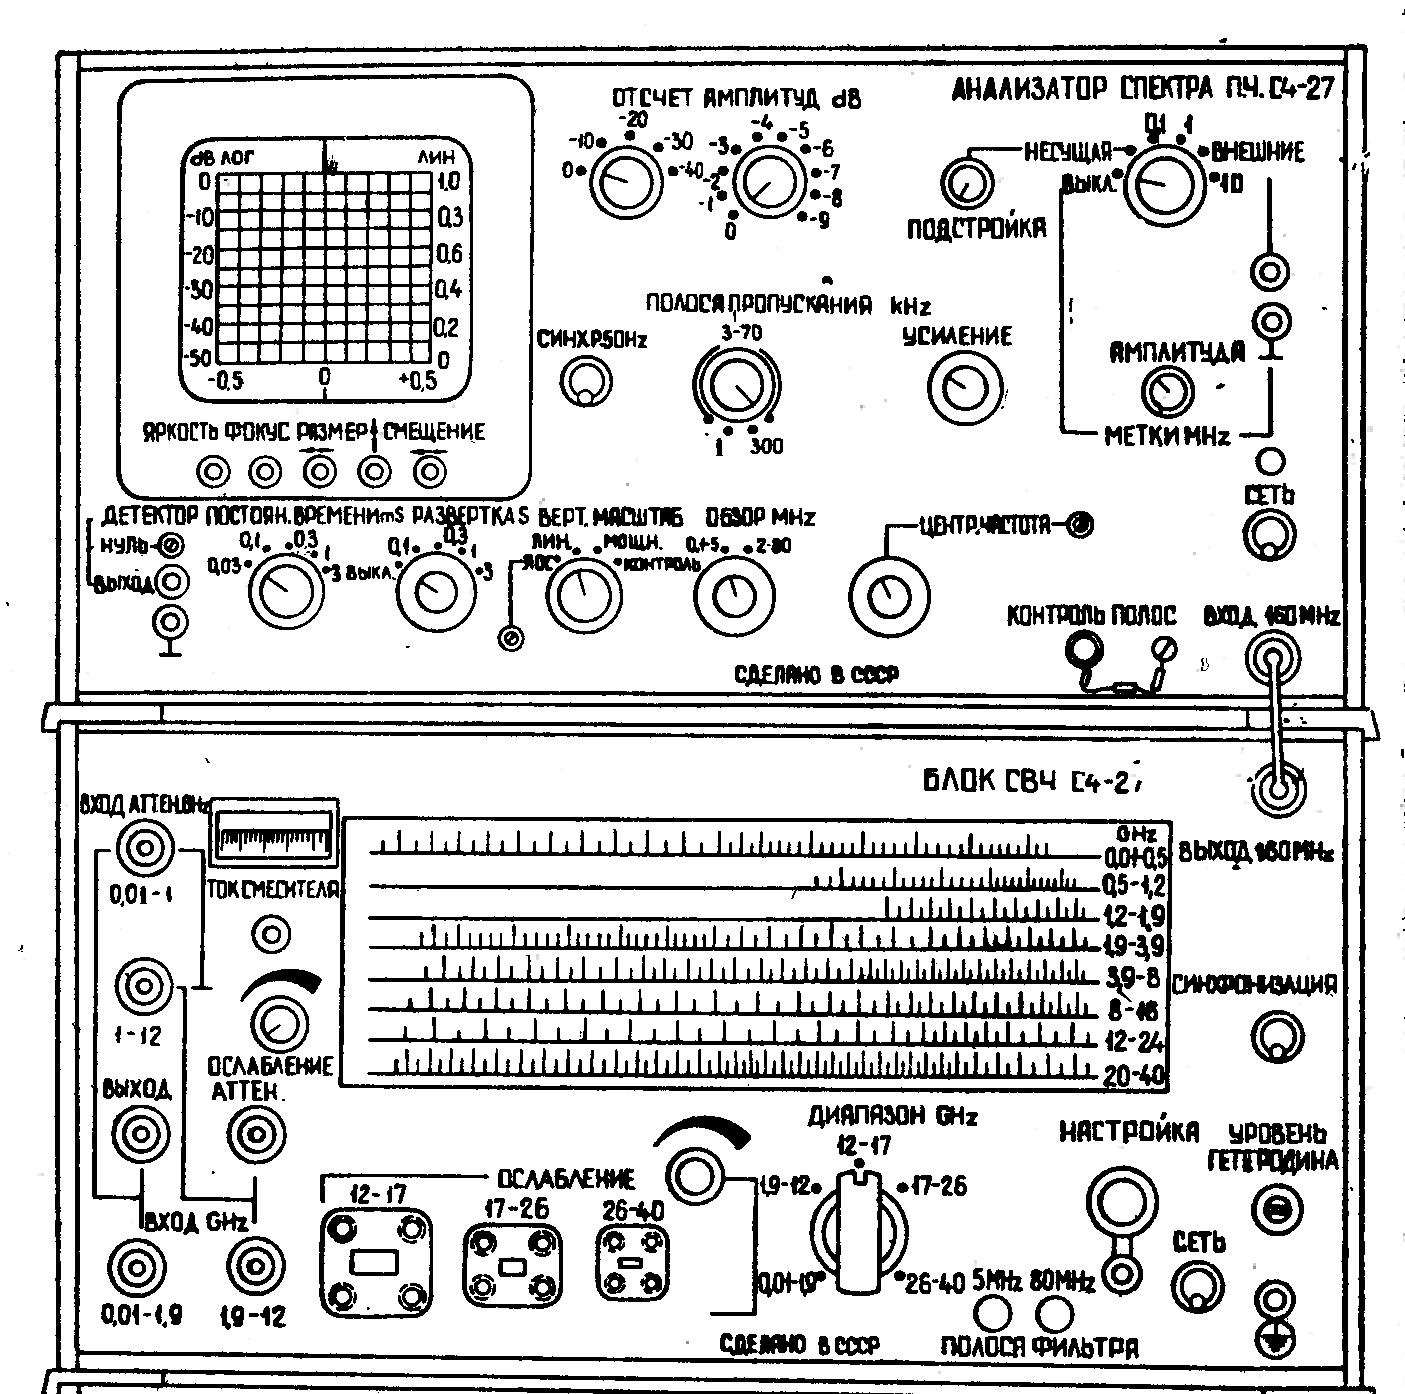
\includegraphics[width = \textwidth]{images/s4-27.png}
        \caption{Анализатор спектра С4-27}
        \label{figa}
    \end{figure}

	Анализатор спектра С4-27 предназначен для исследования спектров периодически повторяющихся импульсов и непрерывных сигналов. Диапазон частот прибора от 0,01 до 39,6~ГГц с разбивкой на пять поддиапазонов: 0,01~--~1,9; 1,9~--~12; 12~--~17; 17~--~26; 26~--~39,6~ГГц. Прибор обеспечивает свои характеристики после времени прогрева не менее одного часа, но при широкой полосе обзора, когда не требуется высокая точность измерений достаточно 10 минут. На вход смесителей~-- непосредственно на ВХОД GHz, для волноводных~-- в крайнем положении ручки ОСЛАБЛЕНИЕ нельзя подавать сигнал мощностью более 1~мВт. В этом случае сигнал на прибор следует подавать только через аттенюатор прибора или внешний аттенюатор. Максимальная мощность, подаваемая на входные аттенюаторы приборы не должна превышать 0,2~Вт. Для клистрона с волноводным выходом $23\times10\,$мм, используется диапазон шкалы 1,9~--~12~ГГц частотами > 6,52~ГГц.  
	
	Ручкой НАСТРОЙКА находят диапазон, в котором есть отклики сигнала, выставляя на блоке СВЧ частоту в нужном диапазоне на некоторое деление, затем переходят в режим меток 10 МГц на блоке ПЧ, после чего отсчитывают количество меток от центральной метки до исследуемого сигнала на экране и вычитают или прибавляют полученное значение к значению по шкале блока СВЧ. Точность такого измерения составляет 10~МГц. Её можно повысить, если уменьшить полосу пропускания исследуемого сигнала и воспользоваться метками с шагом 0,1~ГГц и 1~ГГц.
	
	\subsubsection{Аттенюаторы}
	
	В работе используются 3 коаксиальных аттенюатора. Так как с самого начала уровень выходной мощности не известен, то требуется последовательно подключая аттенюаторы на 10 дБ, 6 дБ и 3 дБ, провести измерения уровня мощности до тех пор пока он не окажется в пределах 10 мВт, также аттенюаторы следует применить при измерении частоты по анализатору спектра, но здесь важно следить за тем, чтобы сигнал можно было отличить от шума. 
    
    { \color{gray}
	\subsection{Проведение измерений}

	\subsubsection{Определение зон генерации, рабочей частоты и добротности}
	
	\begin{enumerate}
		\item Проверьте, что на рабочем столе присутствуют 3 соединительных провода, клистрон, блок питания, коаксиальный кабель, 2 волноводно-коаксиальных переходника, волновод (сечением больше либо равный сечению выходного фланца клистрона), термисторная головка для данного волновода, измеритель мощности, вольтметр (или мультиметр).
		\item Соберите установку по схеме измерений \ref{sch2}. Включите измеритель мощности и дайте ему прогреться. Подключите к нему термисторную головку, и соедините её с волноводом нужного сечения или сразу с волноводно-коаксиальным переходником. Переходник соедините с аттенюатором пока на 10 дБ. Аттенюатор соедините с коаксиальным кабелем, а коаксиальный кабель с клистроном.
		\item Включите блок питания и проверьте, что напряжения катода и отражателя соответствуют номинальным напряжениям таблицы \ref{tab1}. Выключите блок питания.
		\item Выставьте 0 на измерителе мощности с помощью кнопок грубой и точной настройки (первая и вторая кнопка соответственно, в режиме грубой настройки воспользуется винтом и добейтесь максимально близкого к 0 значения, затем воспользуйтесь кнопкой точной настройки), нажмите третью кнопку для того чтобы перейти в режим измерений.
		\item На блоке питания переключите тумблер вольтметра 5 в режим напряжений катода. Включите блок питания. Когда показания вольтметра начнут падать (подождите 90~c.), начнётся генерация клистрона. Переключите тумблер 5 в режим напряжений отражателя и проверьте наличие генерации во всём диапазоне от 90 до 190~В, если показания измерителя мощности слишком малы во всём диапазоне напряжений, измените аттенюатор на другой с меньшим затуханием. Если и это не дало результата, уберите аттенюатор. Обычно в этом случае в центрах зон генерации показания ваттметра достигают нескольких мВт.
		\item Занесите в таблицу \ref{zones1} границы зон генерации $U_{r, min}$ $U_{r, max}$, центры зон генерации $U_{r, \text{ц}}$ по вольтметру 10 или внешнему вольтметру и количество зон генерации в данном диапазоне напряжений отражателя. Запишете также напряжения на катоде в этих точках. 
		\begin{table}[h]
			\center
			\caption{Определение зон генерации}
			\label{zones1}
			\begin{tabular}{|c|c|c|c|c|}\hline
				\multirow{2}*{$U_0,~\text{В}$} & \multicolumn{3}{|c|}{$|U_r|,~\text{В}$} & \multirow{2}*{n} \\ \cline{2-4}
				& минимум & центр & максимум & \\
				\hline
				\multirow{2}*{} &  &  & &  \\ \hline
				&  &  &  & \\ \hline
			\end{tabular}
		\end{table}
		\item Используя формулу \eqref{eq:n} для напряжений в центрах зон генерации определите номера полученных зон.
		\item Отсоедините коаксиальный кабель с аттенюатором от переходника к термисторной головке и подсоедините его ко входу анализатора спектра 1,9~--~12~ГГц через аттенюатор 10 дБ. Ручкой настройка найдите сигнал. Меняя аттенюаторы и ручкой ТОК СМЕСИТЕЛЯ, добейтесь максимального уровня сигнала.
		\item Наблюдая спектр на экране анализатора, определите наименьшую частоту~-- это и будет основная частота клистрона.
		\item Изменяя напряжение на отражателе снимите зависимость частоты от напряжения отражателя в пределах зоны, которая полностью лежит в диапазоне изменений напряжений отражателя. Занесите данные в таблицу \ref{freqs1}.
		\begin{table}[h]
			\center
			\caption{Определение основной частоты и добротности}
			\label{freqs1}
			\begin{tabular}{|c|c|c|c|c|}\hline
				$U_0,~\text{В}$ & $|U_r|,~\text{В}$ & $f,~\text{ГГц}$ & $f_0,~\text{ГГц}$ & $Q$ \\ \hline
				\multirow{7}*{}
				&& &
				\multirow{7}*{}&\multirow{7}*{}\\ \cline{1-3}
				&& &&\\ \cline{1-3}
				&& &&\\ \cline{1-3}
				&& &&\\ \cline{1-3}
				&& &&\\ \hline
			\end{tabular}
		\end{table}
		\item Используя формулу \eqref{eq:Q} определите добротность клистрона.
	\end{enumerate}

    \newpage
    \section*{Список использованных источников}
    
    \begin{enumerate}
	    \item Вальднер, О. А. Техника сверхвысоких частот~/ О.~А.~Вальднер, О.~С.~Милованов, Н.~П.~Собенин.~--- Москва : Атомиздат, 1974.~--- 232~c.
	    \item Трубецков, Д. И. Лекции по сверхвысокочастотной электронике для физиков. В 2 т.~/ Д.~И.~Трубецков, А.~Е.~Храмов.~--- Москва : Физматлит, 2003.~--- Т. 1.~--- 496~с.
	    \item Федоров, Н. Д. Электронные приборы СВЧ и квантовые приборы~/ Н.~Д.~Федоров.~--- Москва : Атомиздат, 1979.~--- 288~c.
	    \item Вайнштейн, Л. А. Лекции по сверхвысокочастотной электронике~/ Л.~А.~Вайнштейн, В.~А.~Солнцев.~--- Москва : Советское радио, 1973.~--- 400~c.
    \end{enumerate}
}
\end{document}